%
%  HOW TO BUILD TOOLMAP DATAMODEL
%
%  Created by Lucien Schreiber on 2013-02-19.
%  Copyright (c) 2013. All rights reserved.
%

\documentclass[a4paper, 12pt]{article}
\usepackage{crealp-report}
\usepackage{upquote} %to force Latex not substitute ' by `
\usepackage{tocbibind}
%\usepackage{natbib}

\begin{document}
\crealptitle {Tutorial} {How to create a ToolMap datamodel using TmDmCreator} {Lucien Schreiber} {lucien.schreiber@crealp.vs.ch}
\tableofcontents
\pagebreak

\section{Introduction}
This tutorial explains how to create a project ToolMap manually. This approach has the following advantages:
\begin{enumerate}
  \item It ensures the IDs used
  \item It generates a multilingual model
  \item It allows better monitoring of model changes
\end{enumerate}
The main disadvantage of this approach is the lack of user interface as well as the need for the user to have some knowledge of SQL. Finally, this approach has been developed to meet the need for rigor in the management of the geological data model.


\section{Conceptual Workflow}
The diagram shown in figure~\ref{fig:conceptual-workflow} illustrates the proposed workflow. User edits the user\_structure.sql and user\_content.txt files. These files as well as base\_structure.sql are used by the software TmDmCreator to produces either:
\begin{enumerate}
  \item	a SQL file defining the project (output 1)
  \item	a ToolMap project (output 2)
\end{enumerate}

\begin{figure} [htbp]
	\centering
    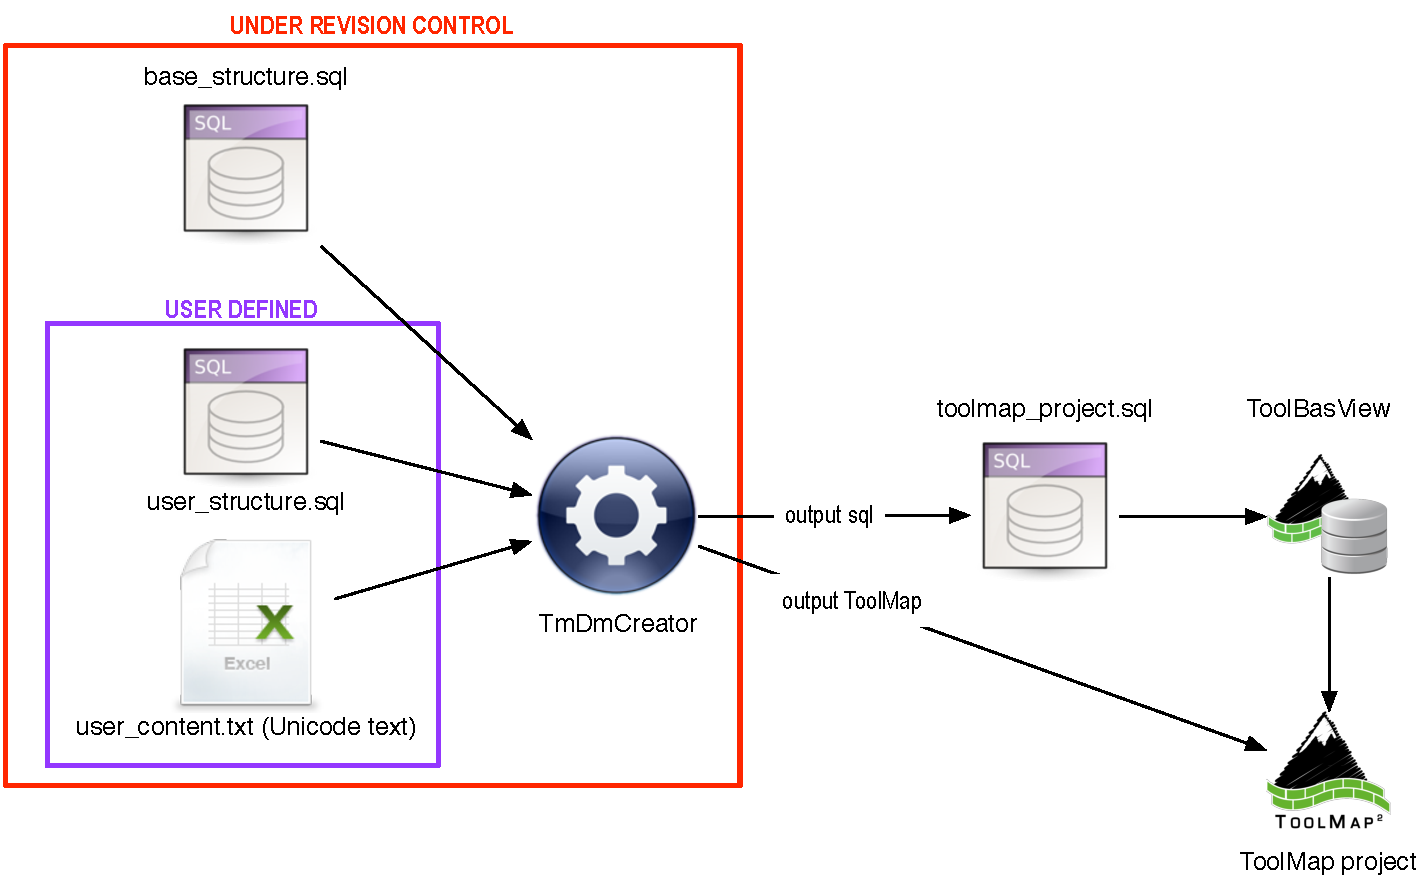
\includegraphics[width=1\textwidth]{img/workflow.pdf}
    \caption{Conceptual workflow}
    \label{fig:conceptual-workflow}
\end{figure}



\section{Data needed}

\section{Preparing user data}

\subsection{Layers}

\subsection{Objects}

\subsection{Attributes structure}

\subsection{Value domain of the attributes}


\end{document}
